% !TEX encoding = UTF-8
% !TEX program = pdflatex

% This is "sig-alternate.tex" V2.0 May 2012
% This file should be compiled with V2.5 of "sig-alternate.cls" May 2012
%
% This example file demonstrates the use of the 'sig-alternate.cls'
% V2.5 LaTeX2e document class file. It is for those submitting
% articles to ACM Conference Proceedings WHO DO NOT WISH TO
% STRICTLY ADHERE TO THE SIGS (PUBS-BOARD-ENDORSED) STYLE.
% The 'sig-alternate.cls' file will produce a similar-looking,
% albeit, 'tighter' paper resulting in, invariably, fewer pages.
%
% ----------------------------------------------------------------------------------------------------------------
% This .tex file (and associated .cls V2.5) produces:
%       1) The Permission Statement
%       2) The Conference (location) Info information
%       3) The Copyright Line with ACM data
%       4) NO page numbers
%
% as against the acm_proc_article-sp.cls file which
% DOES NOT produce 1) thru' 3) above.
%
% Using 'sig-alternate.cls' you have control, however, from within
% the source .tex file, over both the CopyrightYear
% (defaulted to 200X) and the ACM Copyright Data
% (defaulted to X-XXXXX-XX-X/XX/XX).
% e.g.
% \CopyrightYear{2007} will cause 2007 to appear in the copyright line.
% \crdata{0-12345-67-8/90/12} will cause 0-12345-67-8/90/12 to appear in the copyright line.
%
% ---------------------------------------------------------------------------------------------------------------
% This .tex source is an example which *does* use
% the .bib file (from which the .bbl file % is produced).
% REMEMBER HOWEVER: After having produced the .bbl file,
% and prior to final submission, you *NEED* to 'insert'
% your .bbl file into your source .tex file so as to provide
% ONE 'self-contained' source file.
%
% ================= IF YOU HAVE QUESTIONS =======================
% Questions regarding the SIGS styles, SIGS policies and
% procedures, Conferences etc. should be sent to
% Adrienne Griscti (griscti@acm.org)
%
% Technical questions _only_ to
% Gerald Murray (murray@hq.acm.org)
% ===============================================================
%
% For tracking purposes - this is V2.0 - May 2012

\documentclass{sig-alternate}
\usepackage[utf8]{inputenc}
\usepackage{listings}
\usepackage{url}
\usepackage{footnote}
\usepackage{color}

\begin{document}
%
% --- Author Metadata here ---
\conferenceinfo{AGERE!}{'15 Pittsburgh, Pennsylvania, USA}
%\CopyrightYear{2007} % Allows default copyright year (20XX) to be over-ridden - IF NEED BE.
%\crdata{0-12345-67-8/90/01}  % Allows default copyright data (0-89791-88-6/97/05) to be over-ridden - IF NEED BE.
% --- End of Author Metadata ---

% \title{Towards a portable actor runtime environment}
\title{Akka.js: Towards a portable actor runtime environment}

%
% You need the command \numberofauthors to handle the 'placement
% and alignment' of the authors beneath the title.
%
% For aesthetic reasons, we recommend 'three authors at a time'
% i.e. three 'name/affiliation blocks' be placed beneath the title.
%
% NOTE: You are NOT restricted in how many 'rows' of
% "name/affiliations" may appear. We just ask that you restrict
% the number of 'columns' to three.
%
% Because of the available 'opening page real-estate'
% we ask you to refrain from putting more than six authors
% (two rows with three columns) beneath the article title.
% More than six makes the first-page appear very cluttered indeed.
%
% Use the \alignauthor commands to handle the names
% and affiliations for an 'aesthetic maximum' of six authors.
% Add names, affiliations, addresses for
% the seventh etc. author(s) as the argument for the
% \additionalauthors command.
% These 'additional authors' will be output/set for you
% without further effort on your part as the last section in
% the body of your article BEFORE References or any Appendices.

\numberofauthors{3} %  in this sample file, there are a *total*
% of EIGHT authors. SIX appear on the 'first-page' (for formatting
% reasons) and the remaining two appear in the \additionalauthors section.
%
\author{
% You can go ahead and credit any number of authors here,
% e.g. one 'row of three' or two rows (consisting of one row of three
% and a second row of one, two or three).
%
% The command \alignauthor (no curly braces needed) should
% precede each author name, affiliation/snail-mail address and
% e-mail address. Additionally, tag each line of
% affiliation/address with \affaddr, and tag the
% e-mail address with \email.
%
% 1st. author
\alignauthor
Gianluca Stivan\\
       \affaddr{UniCredit R\&D}\\
       \affaddr{Italy}\\
       \email{Gianluca.Stivan@stud-inf.unibz.it}
% 2nd. author
\alignauthor
Andrea Peruffo\\
       \affaddr{UniCredit R\&D}\\
       \affaddr{Italy}\\
       \email{Andrea.Peruffo@unicredit.eu}
% 3rd. author
\alignauthor Philipp Haller\\
       \affaddr{KTH Royal Institute of Technology}\\
       \affaddr{Sweden}\\
       \email{phaller@kth.se}
\and  % use '\and' if you need 'another row' of author names
% 4th. author
% \alignauthor Lawrence P. Leipuner\\
%        \affaddr{Brookhaven Laboratories}\\
%        \affaddr{Brookhaven National Lab}\\
%        \affaddr{P.O. Box 5000}\\
%        \email{lleipuner@researchlabs.org}
}

\maketitle
\begin{abstract}
Multiple mature implementations of the actor model of concurrency exist. Besides several implementations for Java virtual machines, there are implementations, for example, written in SmallTalk or in C++, targeting native platforms. Recently, runtime environments for platforms such as GPUs have appeared.

However, so far, no full-featured actor runtime environment has allowed actor programs to run, unchanged, on both Java and JavaScript virtual machines. This paper describes our ongoing effort in providing a portable implementation of the widely-used Akka actor runtime.
\end{abstract}

% A category with the (minimum) three required fields
% \category{H.4}{Information Systems Applications}{Miscellaneous}
%A category including the fourth, optional field follows...
% \category{D.2.8}{Software Engineering}{Metrics}[complexity measures, performance measures]

% \terms{Theory}

\keywords{Actors, Portability, Java, JavaScript}

\section{Introduction}

Since its introduction in 1995~\cite{web:js} there has been an increasing interest around JavaScript. Originally, this programming language was developed by Netscape Inc. to provide a lightweight interpreted language to captivate non-professional programmers. Later, thanks to a standardization process started in 1996 with the first release, which continues nowadays up to the sixth version released in June 2015~\cite{web:ecmascript6}, JavaScript has become one of the most popular programming languages on the Web.

It is interesting to analyze the evolution of the language. Before the introduction of Ajax~\cite{web:ajax} JavaScript was mainly used for browser scripting. In 2009 CommonJS~\cite{web:commonjs} and Node.js~\cite{web:nodejs} proposed an ecosystem capable of running JavaScript outside the browser. With the rise of single-page web applications~\cite{} and source-to-source compilers~\cite{}, JavaScript is now being used to power a large variety of projects. 

Despite the improvements made by the JavaScript community, there are several issues that make developing software using JavaScript hard. Working in JavaScript is inconvenient because of its module system (not available before ES6~\cite{web:es6modules}), its weak-typing, the verbose function syntax\footnote{its support for closures is commonly noted as being one of JavaScript\rq{s} redeeming features.}, the late binding\footnote{Early binding allows for static verification of the existence of method-signature pairs}, the lack of static types, the behavior of \emph{this}, the equality/automatic conversion to boolean.

But the biggest issue that JavaScript has is its almost complete lack of support for concurrency. As a language that is by default asynchronous, since all its I/O happens through event-based APIs, it is surprising that the only way to write code is through callbacks (up to ES6) and promises (from ES6 upwards). This has resulted in a lot of code that resembles the so-called callback hell, where the code moves to the right faster than to the bottom, because of all the nested functions.

The actor model has been successfully used to write all kinds of concurrent and distributed applications, ranging from telephone switches, to critical infrastructure services such as Amazon's S3 and so on. As such it would be a perfect fit for JavaScript, but unfortunately there is no widely used or supported implementation of the actor model that targets the JavaScript runtime.

We decided to look to other virtual machine environments and found in Akka a mature framework for the JVM which can be used both from Scala and from Java. Given the existence of Scala.js, a Scala to JavaScript compiler, we started investigating the feasibility of porting the Akka framework to JavaScript.

Unfortunately, as the framework is written today, it is heavily dependent on a number of JVM constructs, semantics and data structures. Fortunately we were able to abstract that complexity away and in this paper we present Akka.js, an implementation of an actor system in Scala.js. To goal of this project is to expose a model and an API identical to Akka, so that Scala developers can reuse transparently knowledge between the client-code (\emph{Browser}) and the server-code.

%
%In 1973, a joint effort between Carl Hewitt, Peter Bishop and 
%Richard Steiger resulted in the Actor Model. Presented in a paper  published in 1973, this revolutionary architecture was, according to its creators, inspired by physics and programming languages such as Simula and LISP. The philosophy at the foundation of this model is that everything is an actor, where an actor is an entity which does exactly three things:
%\begin{itemize}
%\item[-] send messages to other actors 
%\item[-] create a finite number of actors 
%\item[-] react with a defined behaviour to the next incoming message 
%\end{itemize}
%Every actor is identified by an \textit{address}, which uniquely identifies it in the domain. The address is particularly interesting because it introduces the notion of \textit{location transparency}, meaning that the physical location of an actor is unnecessary, as long as an address pointing to it is correct, because the framework mechanism will ensure delivery.

This paper presents our ongoing effort to enable {\em portability} of systems and applications based on actors in Scala~\cite{ActorsInScala}, using the Akka actor-based middleware~\cite{Akka}.

Traditionally, actor-based programs in Scala have been restricted to run on the Java virtual machine~\cite{Lindholm-Yellin}, Scala's main compilation target. This has enabled creating highly-scalable, concurrent and distributed systems powering services provided by Amazon, The Guardian, and BBC, among others.

However, additionally enabling actor-based applications to be deployed on JavaScript runtimes presents numerous advantages. For starter, it brings an arguably very good model, which handles concurrency and fault handling admirably, to a runtime which lacks good support for both. Moreover, it promotes state isolation, which makes reasoning about the application easier for programmers. Finally the message passing abstraction fits incredibly well to all kind of I/O operations that JavaScript provides. WebSockets, WebWorkers, AJAX and DOM Events are all asynchronous and event-based, making a wrapper that forwards events as messages to actors both convenient and simple to use at the same time.

{\em Akka.js} is our effort to provide a full-featured Scala actor framework for JavaScript runtimes. It enables portable actor-based applications,
compiled against the Akka API, to target both the JVM and JavaScript runtimes. Another important goal of the project is seamless
messaging between actors running on JavaScript runtimes (e.g., web browsers) and actors running on JVMs.

Our approach can be divided into two inter-related parts:
\begin{itemize}
\item Porting the original JVM-based implementation of Akka (Akka.JVM in the following) to JavaScript; and
\item Techniques and tools for sharing Scala code between Akka.JVM and Akka.js.
\end{itemize}
\noindent
The second issue is of major importance: the lack of a shared code base would require {\em manual synchronization} of two large code bases, with
corresponding large engineering costs. Moreover, the lack of automatic, compiler-time checks would make it extremely difficult to ensure the
portability of Akka-based programs across Akka.JVM and Akka.js.

The paper proceeds as follows. We first give a brief\newline overview of Akka and its API (\S~\ref{sec:akka}). We then discuss at length the major challenges encountered during the development of Akka.js (\S~\ref{sec:challenges}), which include reliance on JVM constructs (data structures, patterns, and libraries), usage of reflection, blocking APIs, and serialization. We also detail the solutions adopted to circumvent the presented issues. To enable cross compilation, ensuring cross-compatibility between Akka.JVM and Akka.js, we introduce extensions to Scala.js, the Scala-to-JavaScript compiler (\S~\ref{sec:cross-compilation}). Finally, we outline future work and offer a conclusion (\S~\ref{sec:conclusion}).


\section{Related Work}


A source of inspiration was \textit{Scala-js-actors}.
Developed as a semester project by EPFL PhD student Sébastien Doeraene in fall 2013, it was designed as a way to prove Scala-js' real world capabilities.
The code contains a small subset of the entire Akka.JVM codebase, but supports already actors, supervision and fault-tolerancy.
Scala-js-actors was further extended to provide interoperability with an Akka backend through WebSockets and multi-core computation using WebWorkers.


While an amazing piece of engineering, the limits of scala-js-actors are:
\begin{itemize}
\item[-] no relationship with the original Akka codebase
\item[-] no testing suite
\item[-] different semantics from Akka.JVM remote, the Akka module for communicating with remote nodes
\end{itemize}
To elaborate a bit further, the first two points where due to the fact that scala-js-actors was a research project, a proof of concept of the maturity of Scala.js, hence it was not designed with a long-term strategy in mind.
The third point is more vital. Akka.JVM remote is the component that allows different JVMs to seamlessly communicate between them using the same abstraction that one would use for local actors. It's the ultimate implementation of the location transparency concept of the actor model.
Whereas in Akka.JVM the programmer needs only to configure the cluster and there is no perceivable difference between 
remote and local actors (please note that Scala, as Erlang, uses the \emph{a ! msg} notation to denote a message \emph{msg}
being sent to an actor \emph{a}):
\begin{lstlisting}
localActor ! "msg"
remoteActor ! "msg"
\end{lstlisting}
In scala-js-actors configuration is not supported, meaning that the programmer has to take care of the setup
\begin{lstlisting}
// Main
...
WebWorkerRouter.initializeAsRoot()
val workerAddress = 
  WebWorkerRouter
    .createChild("worker.js")
// Child
...
WebWorkerRouter.setupAsChild()
WebWorkerRouter.onInitialized { ... }
\end{lstlisting}
In the above example, \emph{WebWorkerRouter} is necessary because it takes care of routing the messages to the
correct actor, since there is no underlying platform that takes care of it, as it is the case with Akka.JVM remote.
This poses serious problems when it comes to Akka.JVM interoperability, so for these reasons, it was decided 
that it would be beneficial to iterate on the original scala-js-actors codebase and provide a library that 
diverges as little as possible from the original Akka, so that it would be instant or trivial to port Akka 
applications to the browser.
In particular the benefits Akka.js addresses the 3 main concerns about scala-js-actors by providing a 
test suite, a 1-1 ratio with Akka.JVM code and includes in the roadmap full support for akka-remote
semantics.

\section{Akka}\label{sec:akka}

Akka is a library written for the Java Virtual Machine which enables programmers to write
scalable, resilient and responsive applications. It does so by providing a high-level
abstraction built on top of the Actor Model and, although written in Scala, it can be used
from other JVM languages as well.

It was originally created by Jonas Boner, now CTO at Typesafe, but has since evolved to
provide all kinds of abstractions over actors and is included by default in the Scala 
standard library.

Akka provide you a number of advantages:
\begin{itemize}
	\item[-] Simple and high-level abstractions for concurrency and parallelism.
	\item[-] Asynchronous, non-blocking and highly performant event-driven programming model.
	\item[-] Very lightweight event-driven processes (several million actors per GB of heap memory).
	\item[-] Fault tolerance through supervisor hierarchies with ``let-it-crash'' semantics.
	\item[-] Location transparency in distributed environments, pure asynchronous message passing. 
\end{itemize}

So both the aspect of the actor model are covered, the design and development Api that let write concurrent software over the actor abstraction and the runtime library that provide powerful features of error handling and actor's life-cycle management.
\\\\

Moreover actor's model features are sweetly merged into the Object Oriented/ Functional paradigm Scala offer.
To understand how Akka achieve this result we can look at the very first component you have to use while using the library, the ActorSystem.
ActorSystem is an high level abstraction over a container of actors, it is heavy weight and it wrap a Thread Pool to hide the Jvm specific basic concurrency model.
All actors must be spawned within an ActorSystem and so it will be possible to separate different runtime needs even within the same Jvm.
Creating a new ActorSystem is as easy as:
\begin{lstlisting}
val system = ActorSystem create
\end{lstlisting}

Akka actors are containers for State, Behavior, Mailbox, Children and Supervision Strategy and the detached interface that enable to interact with the resto of the world is represented by an Actor Reference (ActorRef).
In practice Akka Actor is a Scala trait which means that is an interface with concrete and abstract members that can be extended by any arbitrary class.
In this case the only abstract member that has to be defined in order to have a concrete instance of an Actor is the receive method.
The signature of the receive method 
\begin{lstlisting}
def receive: PartialFunction[Any, Unit]
\end{lstlisting}
tells us more about the details of the implementation, it is a composable function that will be synchronously applied each time one message is dequeued from the Mailbox.
An actor doesn't needs to explicitly crunch messages as they are automatically processed one by one as long as the Mailbox is not empty.
\\\\

A common practice in Scala is to use Pattern Matching over types so a simple actor that when receive a string ``ping'' notify it in the user console looks like this
\begin{lstlisting}
class PingReceiver extends Actor {
def receive = {
case "ping" => println("Ping message received")
}
}
\end{lstlisting}

Since Actors are not common objects in Scala they need a special syntax to be instantiated.
It is so needed to explicitly spawn the actor from the previously created ActorSystem through a generation property container called Prop, in the Prop object it is possible to specify many detailed option that are not going to be covered within this paper.
\begin{lstlisting}
val actor = system actorOf Props[PingReceiver]
\end{lstlisting}

In order to explicitly send messages to the spawned actor it is possible to use the usual (at least for Erlang developers) \verb|!| bang operator.
\begin{lstlisting}
actor ! "ping"
\end{lstlisting}

In this case we get the expected result that ``Ping message received'' will be printed to the standard output.
To summarize you can find that Akka is actually one of the most idiomatic and appreciated way of writing actor based system in the Java ecosystem.

\section{Portable runtime environment}\label{sec:challenges}

In order to achieve a perfectly portable runtime environment, it is first necessary to understand the semantics of the target. 
JavaScript can run in many different environments, including
\begin{itemize}
\item[-]{Node.js, a JavaScript runtime for server side applications}
\item[-]{Phantom.js, a headless WebKit browser, programmable through APIs}
\item[-]{Rhino, a JavaScript engine running on the Java Virtual Machine}
\item[-]{Browsers, in general}
\end{itemize} 
Fortunately, these environments, albeit not identical, share some common traits, which simplify the process of understanding where to focus the porting effort. One such trait is the \textit{JavaScript's execution model}.

\subsection{JavaScript's execution model}

JavaScript is a dynamic, single-threaded programming language. It provides some functional concepts such as closures and partial support for operating on collections (eg: map, reduce, filter).
JavaScript is also inherently concurrent, since all its I/O operations are asynchronous and event based.
In order to better understand how this affects the development of programs, it is necessary to explicitly specify what we mean when we say \textit{asynchronous event-based I/O}.

JavaScript only has a few ways of interacting with the outside world: one is the Document Object Model, a tree-like structures which represents the HTML of the current web page, another is WebSockets and all the AJAX family which include facilities to communicate to a remote server, and finally there is WebWorkers, a novel standard which allows multiple JavaScript runtimes to be spawned and communicate with one another through message passing.
Every time we interact with one of these components a return value isn't immediately available, but the programmer must register explicit interest in the appropriate event. This is where the event loop comes into play. This event loop is a regular loop which listens for events and subsequentially executes the corresponding handler that the programmer has specified, using a callback mechanism.

\subsection{Akka.js}

Akka.js is the core project of this thesis and builds on \textit{scala-js-actor}, a previous PhD 
semester project developed at École polytechnique fédérale de Lausanne by Sébastien Doeraene. 
The original codebase has been pretty much rewritten from scratch to more closely mimic the 
Akka.JVM code, but Doeraene's work has served as a great source of inspiration for this thesis.
What Akka.js really is, is a partial port of the Akka ecosystem to Scala.js, which allows 
Akka programs to run directly everywhere JavaScript is available. It achieves this by 
replacing all the Java Virtual Machines dependencies with their JavaScript counterparts 
while keeping the semantics of the library unchanged.
\\\\


The project also provided some interesting challenges, some of which are mentioned below.
The biggest problem that arose was the heavy dependency on JVM code that Akka.JVM has. JVM code is intertwined with code that
can be shared with Akka.JS and there is no easy way to remove it. Examples of such dependency are threads, JVM data structures
and JS semantics differing from the JVM.
The problem was solved in two ways. First, code was divided in two directories, one with JavaScript specific code, another with
code that is shared with Akka.JVM. Second, the JavaScript specific code was rewritten from scratch to allow Akka to run in JavaScript 
runtimes with the same semantics as in the Java Virtual Machine.
\\
A further problem which was encountered during the development of Akka.js was due to the reflection usage on the JVM. Reflection is
a feature of the Java SDK which allows a programmer to inspect an object at runtime and interact with it in ways that would not 
normally be possible. Unfortunately, support for such features is non-existent in the JavaScript runtime, so it was necessary to
develop a custom solution. A subset of the \emph{java.lang.reflect} APIs was developed, which is semantically identical to the JVM
counterparts. A proposal has also been submitted to the Scala.js core team, to allow for a tighter integration with the compiler. 
If the proposal is accepted, this will result in a superior kind of integration and it will be possible to definitely eliminate the
last hacky bits in the code.
\\
Finally, the usage of JVM's blocking APIs in the test code has proven to be quite the source of difficulties. Given its single threaded
nature it is not normally possible to block in a JavaScript runtime, effectively rendering the available Akka test code unusable.
The limitation was circumvented by writing a custom event loop dispatcher that allows for blocking operations. Normally this would result
in a deadlock, but given the asynchronous nature of Akka, the only blocking code is the test itself, so it ends up working just fine.

\subsection{Scala.js}

Scala.js is an alternative compiler for the Scala language that instead of targeting the Java Virtual Machine and producing bytecode targets Javascript.
As many other efforts in and out the JVM (GWT, CoffeeScript, ...) the goal here is to provide an higher-level language to Javascript, in order to achieve easy code reusability, abstranctions and tooling.
Moreover one key point of the project is Javascript interoperability, in both directions, plain Javascript libraries could be wrapped from Scala interfaces and used in Scala.Js and Scala.Js could expose to Javascript defined APIs.
The project actually feature 100% of the Scala code coverage, a lot of usefull facades on the most popular JavaScript libraries, 
Since most of the compilers to Javascript loose is performance it is important to say that fully optimized code execute is almost comparable timing.


\section{Cross compilation}\label{sec:cross-compilation}

As long as Akka project is very active we face the problem of a diverging the code base since the very first versions of Akka.js.
The analysis of the key differences highlights these conflicts:
\begin{itemize}
	\item[-] Semantic differences on components usable in a JavaScript environment
	\item[-] Java API partially implemented in Java we don't want to support
	\item[-] Missing annotations to expose functionalities to JavaScript code
	\item[-] A tiny number of small hacks used to keep the developer API very clean (mostly reflection-based)
	\item[-] Java data structures
\end{itemize}
Considering the advantages of having a project that can be compiled reusing more than 80% of the original code it was choosen to adopt some strategies in order to have as much as possible a "non intrusive" patching of most of the sources.
\\
If in a file there are implementations that do not conform to Javascript Virtual Machine semantics the implementations and interfaces will be splitted in different files, use just the interfaces and PR the modification to upstream Akka.
Since Java API is hard-wired into interfaces it will be dropped at compile time using a compiler plugin.
Using a compiler plugin as per Java API solution needed annotations will be patched directly on AST at compile time.
The number of hack are hacked themselves case-by-case.
Analyzing data structures used all around in Akka it must be considered that:
\begin{itemize}
	\item[-] Akka was developed with JVM, concurrency and performances in mind.
	\item[-] standard Scala collection library was designed for providing an excellent developer experience and a consistent fully functional API across different kind of collections, this unfortunately result in bad performances.
\end{itemize}
The obvious conclusion is that the collections used all around in Akka code are part of the extremely efficient Java standard library.
When the porting started the interoperability between Java standard library and Scala.Js was limited to a subset of the Arrays manipulation functions.
Instead of changing data structures into the Akka standard library it was chosen to extend the support of Java collections into Scala.Js itself.
Having in mind that Javascript is single-threaded and synchronous we don't have to pay attention in supporting concurrency safe data structures as long as this property is intrinsically provided by the runtime.
Collections were therefore implemented as binding on pure Scala data structure developed respecting pedantically the documentation(JavaDocs) of the JDK.
This result in an extensive improvement of the Scala.Js provided inter-compatibility layer.
Nowadays all the Java data structures used by Akka library are available in the Scala.Js world with the exception of the ``thread-blocking'' ones which will totally compromise the functionality of the Akka system and therefore are not meaningful on a Javascript VM.

\section{Related work}\label{sec:related}

The Clojure language~\cite{Halloway09} supports CSP-style programming using its
core.async library. This library is also supported by
ClojureScript~\cite{ClojureScript}, a compiler for Clojure that targets
JavaScript. The main difference to our effort is the fact that core.async is
implements the CSP model, whereas Akka.js implements the actor model.

Jetlang. (See \url{https://code.google.com/p/retlang/} and \url{https://github.com/jetlang}) are two high performance threading libraries written for C\# and Java. They do not support remoting, but are optimized for in-memory message passing. They support sequential delivery using an interface called IFiber.

Fantom. (See \url{http://www.fandev.org/}) Fantom is a high level language with support for actors. It was designed with portability in mind and Fantom programs can seamlessly run on the JVM and the .NET CLR. Among other goals of the programming language there are: elegant APIs, modularity, support for OOP and FP and declarative programming. Fantom also has support for JavaScript runtimes.

The Reactive Extensions model~\cite{Meijer12} has been ported from .NET to
many other runtimes, including Java (RxJava by NetFlix) and JavaScript (RxJS
by Microsoft). In contrast to Akka.js, these libraries are not intended to
enable code written in one language to be run on another platform; instead,
each library implements the same programming model on different runtimes in a
way that is more or less compatible with the original .NET implementation.
Moreover, the programming model differs from the actor model, e.g., concurrent
processes are not first class.


\section{Potential use cases}\label{sec:usecases}

There are many potential uses cases which demonstrate why Akka.js can be extremely beneficial to the browser, introducing a new way of thinking about interaction in JavaScript environments. The following examples illustrate
potential scenarios where such library could be successfully employed.
\\\\
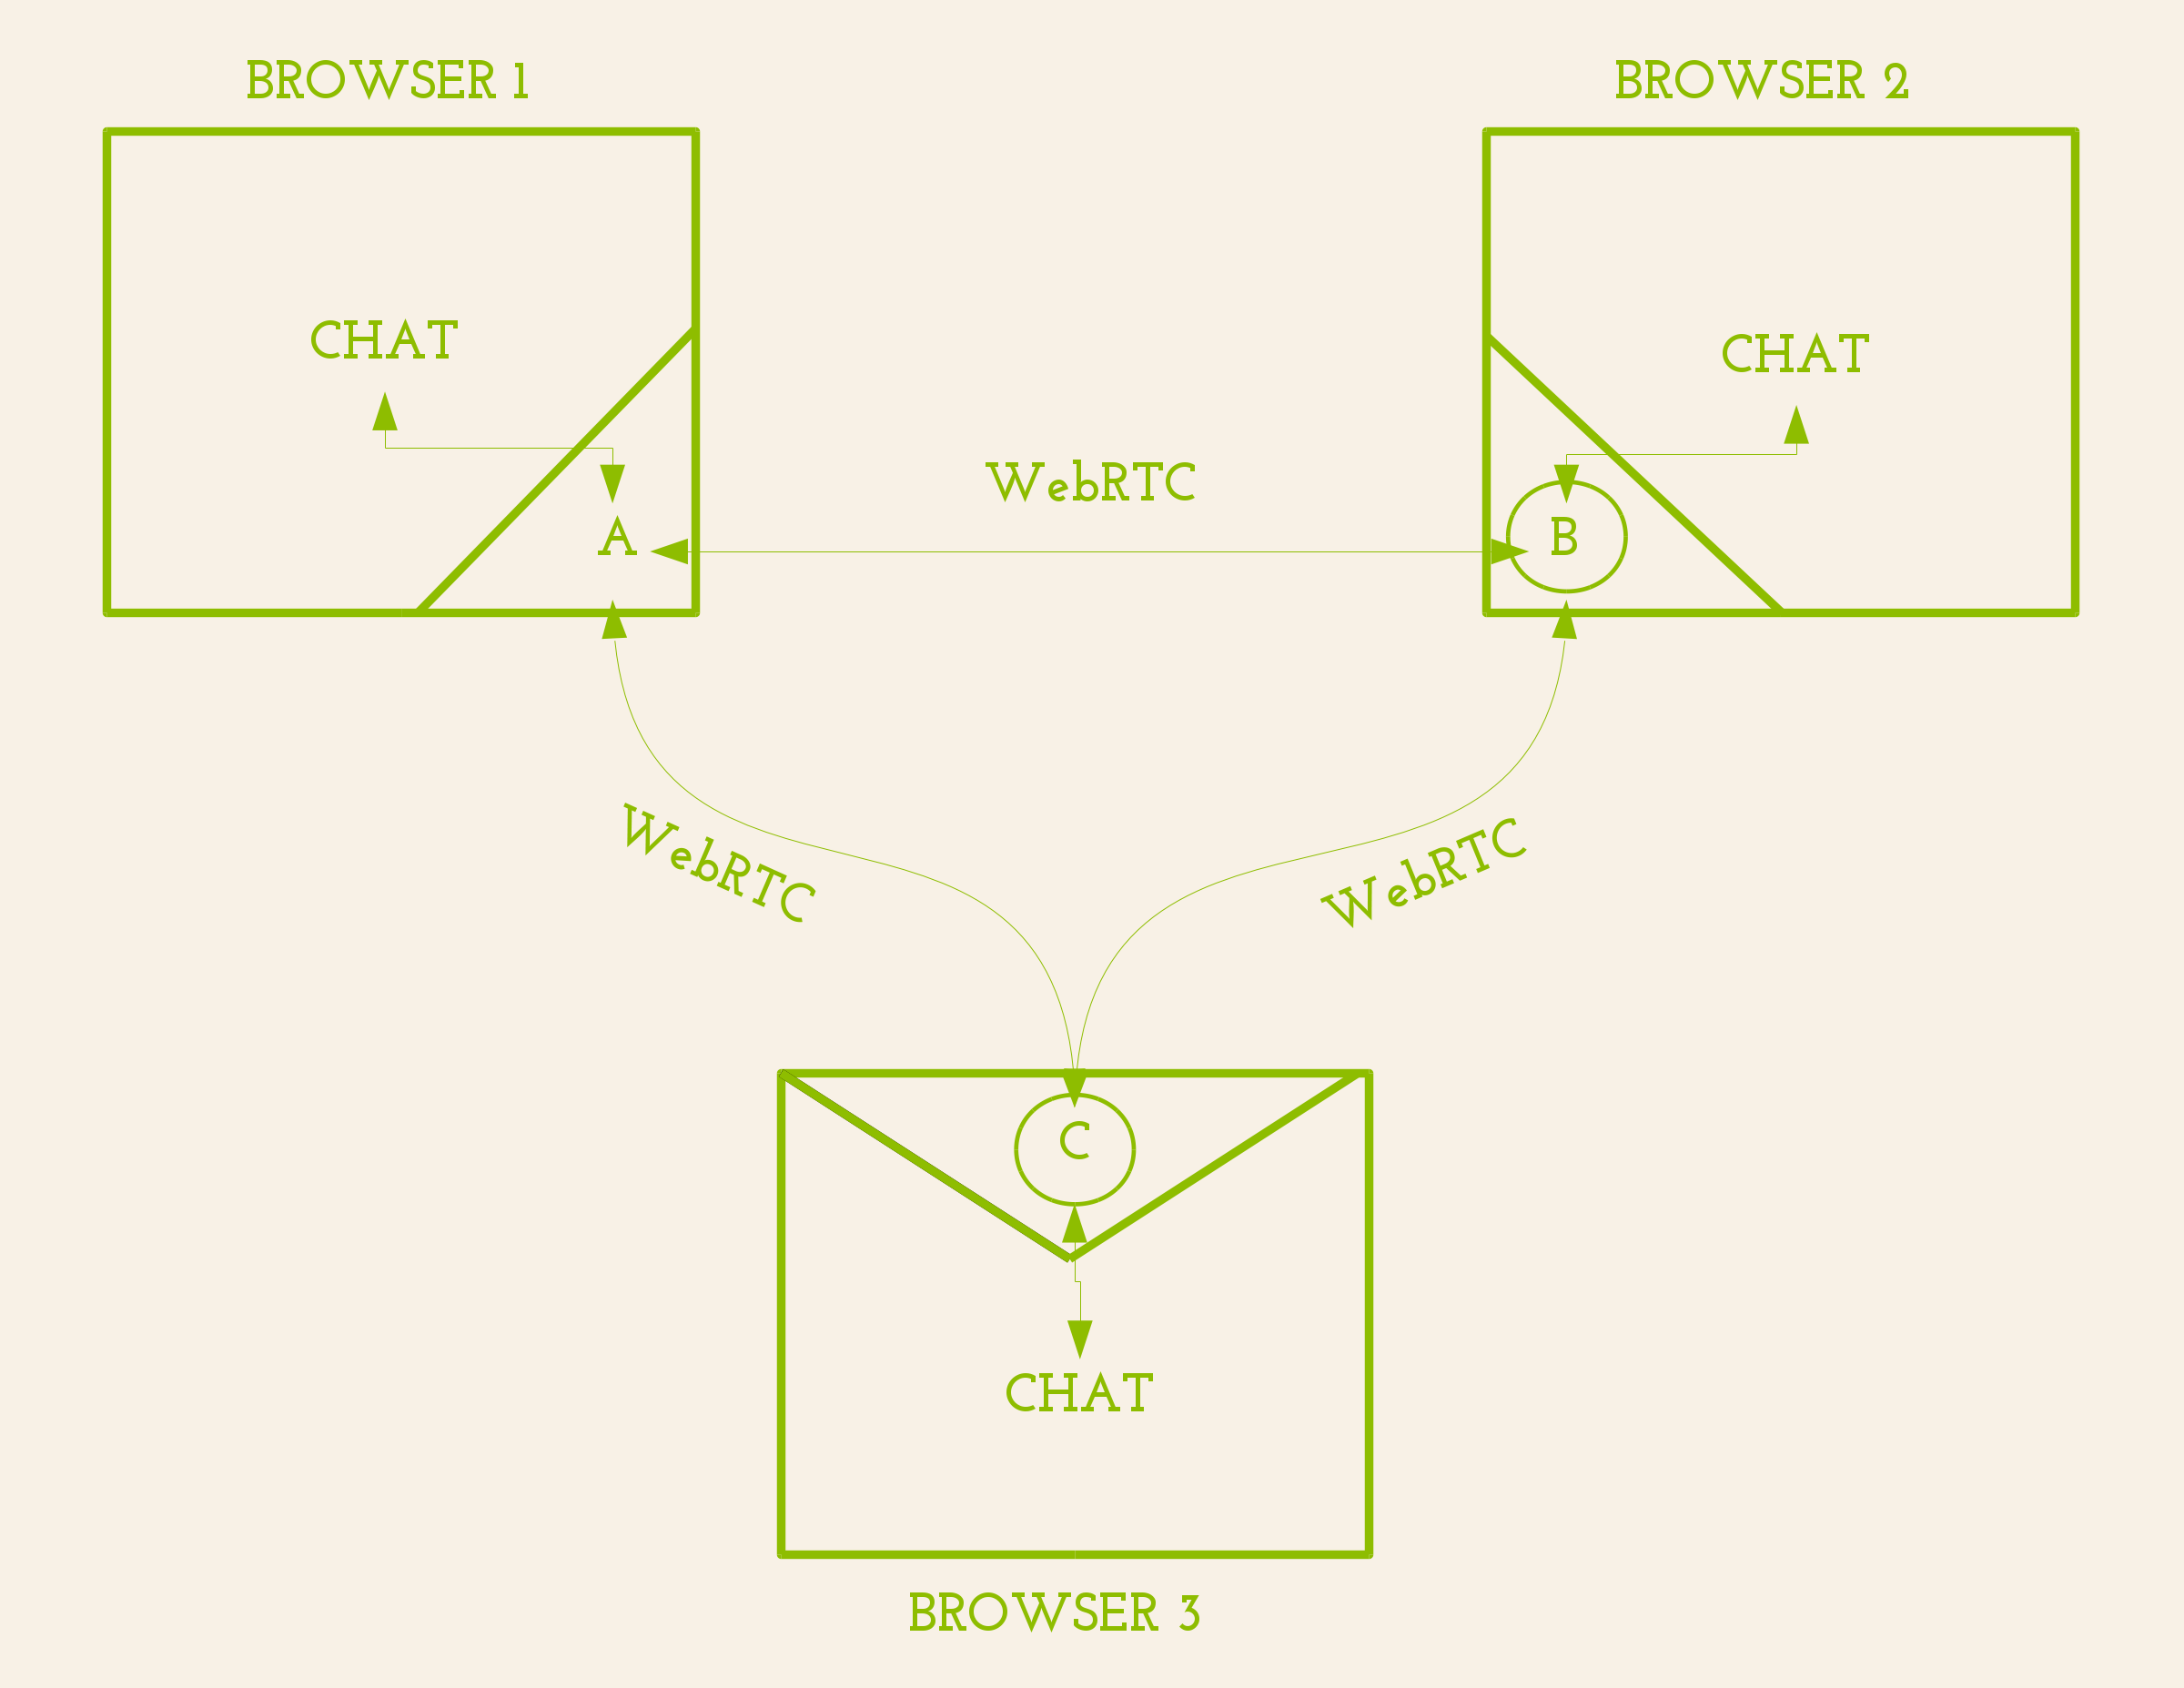
\includegraphics[scale=0.5]{1.png}
\\\\
In this first scenario, a distributed application can be devised using WebRTC as a transport layer.
WebRTC is a technology that allows applications to exploit the benefits of peer-to-peer, from inside
the browser. Given that Akka.js has built-in routing and works by message passing, it would be
possible to abstract away all the complexity from WebRTC and present to the programmer a cluster of
actors which appears local but instead is running in the nodes of a peer-to-peer network.
\\\\
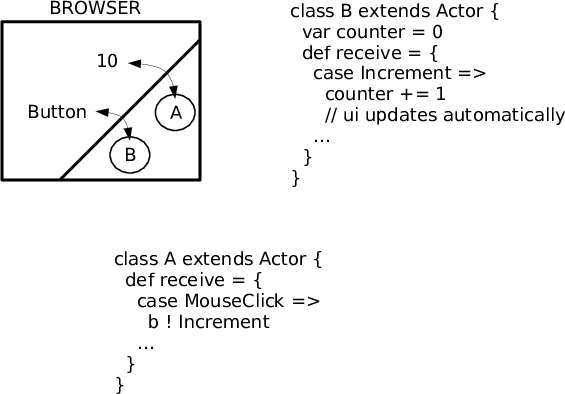
\includegraphics[scale=0.5]{2.png}
\\\\
In the second scenario, a new user interface framework could be developed by exploiting the event-driven
architecture of the browser. All user interactions in the browser happen through so called \emph{events}
which can be handled by the programmer. These events could be wrapped and sent to actors as messages,
transforming all the interactions into one single actor system.
\\\\
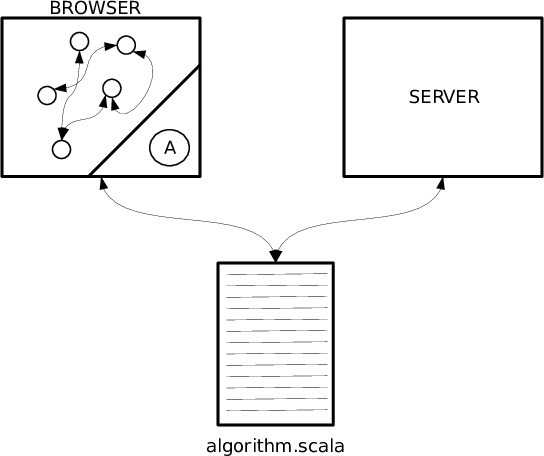
\includegraphics[scale=0.5]{3.png}
\\\\
The third example is potentially interesting for didactic purposes. It is often difficult to picture 
exactly how an algorithm works just by looking at the code. Many algorithms are also implemented
in Akka.JVM, so it would be interesting to insert some barriers into the algorithm which update a 
GUI showing the step-by-step inner workings of the code.
\\\\
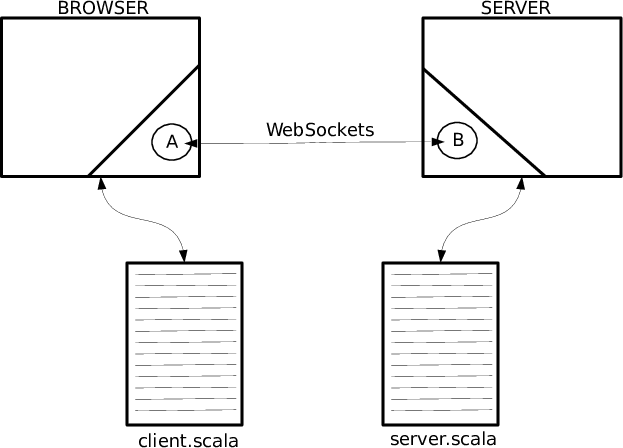
\includegraphics[scale=0.5]{4.png}
\\\\
This fourth example depicts a bi-directional communication channel. Akka.js serves really well as an abstraction layer
that can unite all the different communication protocols. In this case, a frontend application written in Akka.js
can seamlessly interact with a JVM backend running Akka.JVM. The advantage is a unique approach to coding and 
the benefit of needing to master only one language, instead of continuously switching from JavaScript to Scala/Java.
\\\\
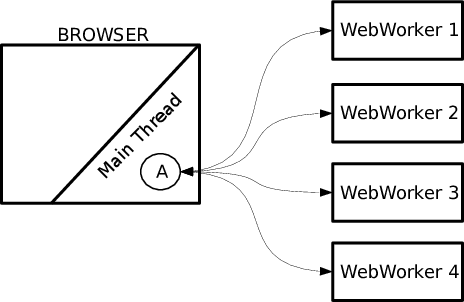
\includegraphics[scale=0.5]{5.png}
\\\\
In this final scenario, Akka.js abstracts away the complexity of dealing with WebWorkers. As mentioned before, WebWorkers
are a set of API allowing multicore in the browser. Unfortunately because it is only possible to interact with WebWorkers 
through message passing, it is usually less than trivial to manage everything with JS and a programmer needs to worry
about serializing and unserializing messages. Akka.js simplifies the approach, in the sense that the programmer can use
the architecture he's already familiar with and Akka.js automatically deals with the low-level components of the WebWorkers
without exposing any of its complexity.

\section{Conclusion and future work}\label{sec:conclusion}

A project was presented, which focuses on cross-compiling Akka to JavaScript, effectively enabling Akka programs to run in different 
JavaScript runtimes (browsers, Node.js and Phantom.JS to name a few).
Akka.js leverages the ubiquity of JavaScript and empowers a whole new set of complex abstractions to be easily managed from one
unique interface, thanks to the elegance of the Actor Model. Different use cases where presented which explain how the project
has practical use cases and can already be used to solve real world problems.
Moreover, as the Akka project is evolving and turning from a simple implementation of the Actor Model, to a complex platform
which can support different kind of reactive applications, the potential for the evolution of Akka.js is enourmous.
There are many modules which still compose Akka.JVM and it would be interesting to explore the possibilities that some of them
enable. For instance:
\begin{itemize}
\item[-] Akka Cluster provides a fault-tolerant decentralized peer-to-peer based cluster membership service with no single point of failure or single point of bottleneck.
\item[-] Akka Streams is an implementation of Reactive Streams, which is a standard for asynchronous stream processing with non-blocking backpressure (meaning that data 
are pulled, instead of pushed, to allow for flow control)
\item[-] Akka Typed is an extension providing statically typed actors
\end{itemize}
In conclusion, Akka is a mature project with strong potential and Akka.js is a first step to harnessing this capability to 
improve the way software is written for the web.

%\end{document}  % This is where a 'short' article might terminate

%ACKNOWLEDGMENTS are optional
\section{Acknowledgments}
This section is optional; it is a location for you
to acknowledge grants, funding, editing assistance and
what have you.

%
% The following two commands are all you need in the
% initial runs of your .tex file to
% produce the bibliography for the citations in your paper.
\bibliographystyle{abbrv}
\bibliography{sigproc}  % sigproc.bib is the name of the Bibliography in this case
% You must have a proper ".bib" file
%  and remember to run:
% latex bibtex latex latex
% to resolve all references
%
% ACM needs 'a single self-contained file'!
%

% That's all folks!
\end{document}
